\chapter{Architecture and Technologies}

This chapter explains the overall architecture of \textit{TextLens} and the main technologies used to develop it. It describes how the system is divided into several functional layers and discusses the frameworks, libraries, and tools that were chosen to support offline, real-time scene text translation on Android devices.

\section{TextLens Architecture}

\textit{TextLens} is designed as an \textbf{offline mobile application} that performs scene text detection, recognition, translation, and rendering directly on the device itself. To support this workflow, the system is organised into three main layers, namely the UI layer, the application control layer, and the on-device processing layer. This layered structure makes the application more modular, easier to maintain, and also easier to test during development.

\begin{itemize}
    \item \textbf{UI Layer:}  
    The UI layer is the part of the system that the user interacts with. It is responsible for showing the live camera preview, allowing the user to choose the source and target languages, supporting freeze-frame mode, and displaying the translated text in a way that is easy to read.

    \item \textbf{Application Control Layer:}  
    The application control layer manages the main workflow of the system. It coordinates the camera input, decides when OCR should be triggered, keeps track of frame and detection states, handles communication between the different modules, and ensures that the UI and processing components work properly together.

    \item \textbf{On-Device Processing Layer:}  
    The on-device processing layer performs the main computer vision and language processing tasks. These include camera frame acquisition, image preprocessing, text recognition, language translation, text region tracking, and scene text replacement. Since all of these operations are carried out locally on the device, the application is able to continue functioning even when there is no continuous internet connection.
\end{itemize}

\begin{figure}[H]
    \centering
    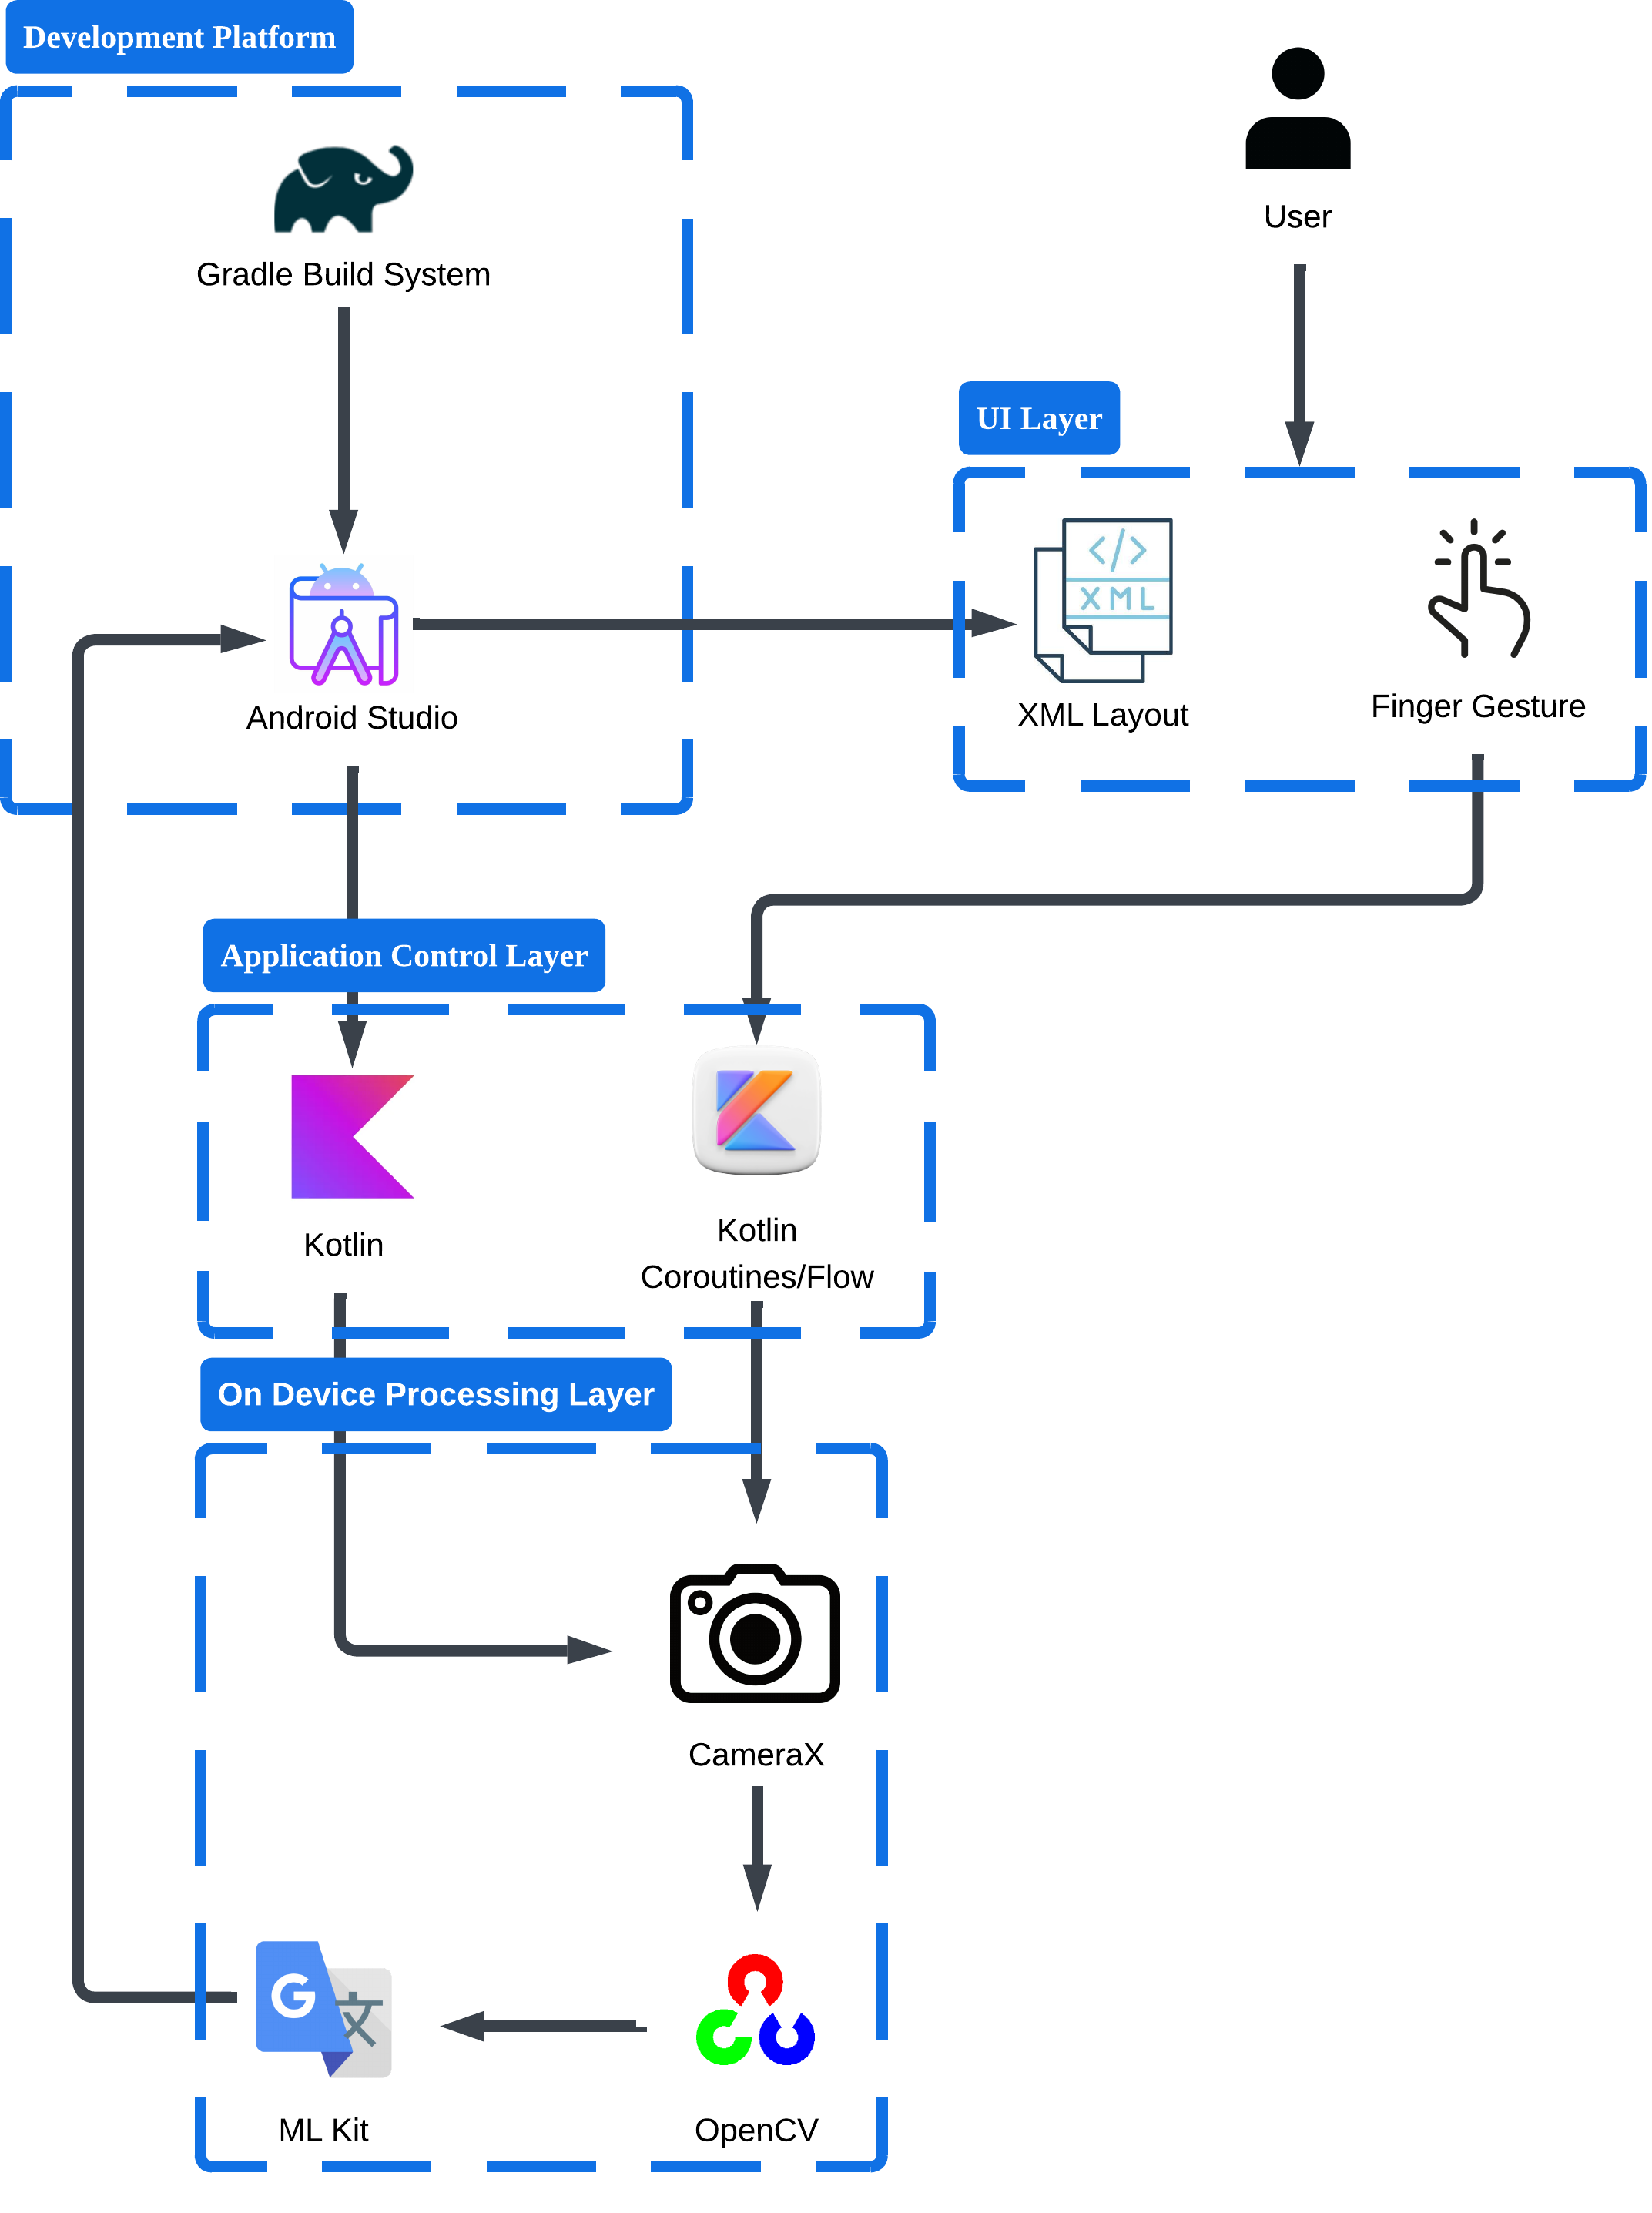
\includegraphics[width=\linewidth]{fig/overview_architecture.png}
    \caption{TextLens architecture overview}
    \label{fig:textlens_architecture}
\end{figure}

\section{Technologies Used}

This section describes the main technologies used in the implementation of TextLens and the rationale for their selection.

\subsection{Frontend and Application Framework}

\subsubsection{Kotlin}
Kotlin is the primary programming language used to develop TextLens. It is officially supported for Android development and provides a concise syntax, strong type safety, and good interoperability with Java-based Android libraries. Its language features also help improve code readability and maintainability.

\subsubsection{XML and Android View System}
The user interface is built using XML layout files together with the Android View system. This approach separates interface design from application logic, making it easier to manage the layout structure, update UI components, and maintain the overall application.

\subsubsection{Android Studio}
Android Studio is used as the main development environment for the project. It provides integrated tools for coding, debugging, dependency management, device emulation, and application packaging, making it suitable for building and testing a full Android application.

\subsubsection{CameraX}
CameraX is used for camera integration and live frame acquisition. It provides a lifecycle-aware API that simplifies camera development and ensures more consistent behaviour across different Android devices. In TextLens, CameraX is used to capture frames for real-time text recognition and translation.

\subsubsection{Kotlin Coroutines and Flow}
Kotlin Coroutines and Flow are used to handle asynchronous and reactive operations in the application. They allow long-running tasks such as OCR, translation, and image processing to run without blocking the UI thread. This helps maintain responsiveness and supports smoother real-time performance.

\subsection{Computer Vision and Language Processing}

\subsubsection{OpenCV}
OpenCV is used for image processing and low-level computer vision operations. In TextLens, it supports tasks such as frame conversion, preprocessing, region handling, inpainting, and image manipulation required for scene text replacement. OpenCV is particularly useful because it provides direct control over pixel-level operations.

\subsubsection{ML Kit Optical Character Recognition (OCR)}
ML Kit's on-device OCR is used to detect and recognize text from camera frames. It provides recognized text together with bounding boxes, which are important for locating text regions in the scene. Since the OCR runs on-device, it supports lower latency and better privacy while allowing the application to operate offline.

\subsubsection{ML Kit Neural Machine Translation}
ML Kit's on-device translation is used to translate recognized text into the user-selected target language. This enables multilingual translation without requiring continuous internet access. The use of on-device translation is an important design choice because it supports the project's objective of offline real-time usability.

\subsubsection{Text Region Tracking}
Text region tracking is used to maintain the position of detected text between OCR updates. This improves the continuity of the displayed translation and reduces the need to run OCR on every frame. Tracking contributes to a smoother and more stable user experience during live camera use.

\subsubsection{Scene Text Replacement}
Scene text replacement is used to render translated text back into the image in a visually coherent way. Instead of simply overlaying translated text on top of the original text, the system removes the original text region and redraws the translated content in the scene. This improves readability and creates a more natural output.

\subsection{Design Approach}

\subsubsection{On-Device Processing}
A key architectural decision in TextLens is the use of on-device processing for the main stages of the pipeline, including OCR and translation. This reduces dependency on cloud services, improves privacy, and allows the application to function in environments with limited or no internet connectivity.

\subsubsection{Modular Pipeline Design}
The application is implemented as a modular pipeline, where major functions such as camera handling, OCR, translation, frame management, and rendering are separated into individual components. This improves code organization, simplifies testing, and makes future enhancements easier to implement.

\subsubsection{Real-Time Mobile Usability}
The technologies used in TextLens are selected not only for technical capability but also for their suitability in a real-time mobile environment. Since the application must process live camera input while remaining responsive, the chosen tools support efficient execution, smooth interaction, and practical deployment on Android devices.
